\documentclass[a4paper, 11pt, oneside, openright, english]{memoir}
\setcounter{secnumdepth}{3} 
\setcounter{tocdepth}{3}

\usepackage[T1]{fontenc}
\usepackage[utf8]{inputenc}

\usepackage{float}
\usepackage{graphicx}
\graphicspath{{./figures/}{./images/}}
\usepackage{rotating}

\usepackage{geometry}
\newgeometry{left=3.5cm,right=3.5cm,bottom=3.5cm,top=3.5cm}

\usepackage{enumitem}
\usepackage{array}

%to make references in the documents
\newcommand{\lbl}[2] {
    \expandafter\gdef\csname item#1\endcsname{#2}%
    \label{#1}#2
}
\newcommand{\uselbl}[2] {\csname item#1\endcsname}
\newcommand{\print}[1] {\ref{#1} \uselbl{#1}\break\par}
\newcommand{\printRef}[1]{\ref{#1}}

%alloy code
\usepackage{listings}
\lstdefinelanguage{alloy}
{
  % list of keywords
  morekeywords={
	assert, pred, all, no, lone, one, some, check, run,
      but, let, implies, not, iff, in, and, or, set, sig, Int, int,
      if, then, else, exactly, disj, fact, fun, module, abstract,
      extends, open, none, univ, iden, seq,
  },
  sensitive=true, % keywords are not case-sensitive
  morecomment=[l]{//}, % l is for line comment
  morecomment=[s]{/*}{*/}, % s is for start and end delimiter
  morecomment=[l]{--},
}

\usepackage{color}
\lstset{
  language={alloy},
  basicstyle=\small\ttfamily, % Global Code Style
  captionpos=b,
  extendedchars=true,
  tabsize=2, 
  columns=fixed, % make all characters equal width
  keepspaces=true, % does not ignore spaces to fit width, convert tabs to spaces
  showstringspaces=false, % lets spaces in strings appear as real spaces
  breaklines=true,
  frame=trbl, % draw a frame at the top, right, left and bottom of the listing
  frameround=false, % make the frame round at all four corners
  framesep=4pt, % quarter circle size of the round corners
  numbers=left,
  numberstyle=\tiny\ttfamily,
  commentstyle=\color{LimeGreen}, 
  keywordstyle=\color{NavyBlue}, 
}

\usepackage[dvipsnames]{xcolor}
\usepackage{hyperref}
\hypersetup{
    colorlinks=true,
    linkcolor=RoyalBlue,
    filecolor=magenta,      
    urlcolor=cyan,
    pdfpagemode=FullScreen,
}
\urlstyle{same}

\begin{document}
	\begin{titlingpage}
	\begin{center}
		
\includegraphics[width=0.3\textwidth]{images/logo_polimi.png}
		
		\vspace{0.25cm}
		
		\LARGE POLITECNICO DI MILANO\\
		
		\vspace{0.2cm}
		
		\Large Computer Science and Engineering
		
		\vspace{0.8cm}
	
		\Huge \textbf{Design Document}
		
		\vspace{0.5cm}
		\huge CodeKataBattle
		
		\vspace{1.5cm}
		\LARGE Software Engineering 2 Project\\
		\Large Academic year 2023 - 2024\\
		\vspace{1cm}
		22 December 2023\\Version 1.0
		\vspace{3cm}
		
		\large
		\begin{minipage}{.4\textwidth}
			\textit{Authors}:\\
			Eliahu Itamar COHEN\\
			Marco GERVATINI\\
                Caterina MOTTI
		\end{minipage}%
		\begin{minipage}{.4\textwidth}
			\raggedleft	
			\textit{Professor}:\\
			Elisabetta DI NITTO\\
			\phantom{placeholder}
		\end{minipage}%
		\begin{minipage}{.1\textwidth}
			\null
		\end{minipage}
	
			
		\end{center}
\end{titlingpage}

	\include{structure/revision_history}

	\tableofcontents

	\pagenumbering{arabic}

	\chapter{Introduction}

\section{Purpose}
The purpose of CodeKataBattle is to provide a platform where students can improve their software development skills by training with peers through code kata battles, a concept inspired by the discipline of martial arts katas, where practitioners repeatedly refine their techniques.
Educators can create battles in which teams of students can compete against each other by developing a solution following a test-first approach.
At the end of each battle, every group is evaluated to create a competition rank that measures each student's performance.
In this document, we will delve into the CodeKataBattle platform, exploring its various features, functionalities, and provide an in-depth analysis of its components.


\subsection{Goals}
Below are presented the goals of CodeKataBattle. Further description will be discussed in section \ref{desc:prodFunc}.
\begin{enumerate}[label=\textbf{G.\arabic*}]
	\item \lbl{goal: manageT} {Educators can create and manage a tournament.}
        \item \lbl{goal: createBad} {Educators can create new badges within a tournament.}
        \item \lbl{goal: createB} {Educators can create a battle within a tournament to which they have access to.}
        \item \lbl{goal: enrollT} {Students can subscribe to a tournament within the specified deadline.}
        \item \lbl{goal: enrollB} {Students can enroll in a battle within their tournaments.}
        \item \lbl{goal: formTeam} {Students can form a team by invite.}
        \item \lbl{goal: rankB} {Students can see their team score in a battle.}
        \item \lbl{goal: listT} {Users can see the list of ongoing tournaments.}
        \item \lbl{goal: rankT} {Users can see all tournaments ranking.}
        \item \lbl{goal: profile} {Users can visualize collected badges of students by visiting their profile.}
\end{enumerate}

\section{Scope}
CodeKataBattle is an online platform that allows students to improve their development skills in a entertaining way. \newline
Educators use the platform to create a code kata battle in which teams can compete against each other. A battle is a programming exercise that the students are expected to solve by following a test-first approach. Each battle belongs to a tournament, that is also created by an educator.
The platform shows to the registered students a list of published tournament and each student can choose to enroll into one of them (before the registration deadline) and form a group by inviting other students. \newline
When the registration deadline expires, the platform automatically creates a GitHub repository containing all necessary code and send the link to all students who enrolled. 
Then the students must push their code in the repository triggering the CKB platform that automatically updates the battle score of the team. \newline
The score is a natural number between 1 and 100. It consist of both an automatic and manual evaluation.  
The automatic evaluation is based on:
\begin{itemize}
    \item functional aspects, measured in terms of number of test cases passed.
    \item timeliness, measured in terms of time passed between the registration deadline and the last commit.
    \item quality level of the sources, extracted thorough static analysis tool that consider multiple aspects selected by the educator at battle creation.
\end{itemize}
When the submission deadline expires, the educators can manually change the score (if needed) and then the platform automatically updates the personal tournament score of each students. These information are then available for all subscribed users. \newline
The CKB platform also include gamification badges, a reward that represent the achievements of individual students. Educators can create a badge by specifying the title and one or more rules that must be fulfilled to achieve it. Each badge can be assigned to one or more students depending on the rules. Earned badges are visible on the personal profile of the student.

\subsection{World Phenomena}
\begin{enumerate}[label=\textbf{WP.\arabic*}]
	\item Students choose which tournament to participate to.
	\item Educators ideate the battle (problem's code, minimum/maximum number of student per group, registration deadline, final submission deadline, additional configuration for scoring).
        \item Students write a solution to the battle and push it in the GitHub repository.
\end{enumerate}

\subsection{Shared Phenomena}
\begin{enumerate}[label=\textbf{SP.\arabic*}]
        \item Educators create a new tournament by inserting on the platform all needed information.
        \item Educators creates badges by inserting on the platform a title and one or more rules.
        \item Users visualize the list of published tournament.
        \item Students joins a new tournament.
        \item Students invites a team member or joins a team.
	\item Educators reviews the score manually for each student.
        \item Users visualize all students' personal profile with their collected badges.
        \item The system send a notification to all students when a new tournament is created.
        \item The system send a notification regarding new battles to all students enrolled in that tournament.
        \item The system send a notification when the final battle rank is available to all students that participated.
        \item The system send a notification when the final tournament rank is available to all students that participated.
\end{enumerate}

\section{Glossary}
\subsection{Definitions}
\begin{center}
	\begin{tabular}{@{}p{0.25\linewidth} p{0.71\linewidth}@{}}
		\toprule
		\textbf{Term} & \textbf{Definition}\\
		\midrule
		Users & Identify both students and educators that are logged in. \\
            Notification & Sent via e-mail, from the system to the recipient. \\
            Code Kata & A set of documents that consist in the description of the project (in which are listed all languages that are acceptable for a solution), the software project, test cases and build automation scripts. \\
		\bottomrule
	\end{tabular}
\end{center}

\subsection{Acronyms}
\begin{center}
	\begin{tabular}{@{}p{0.25\linewidth} p{0.71\linewidth}@{}}
		\toprule
		\textbf{Acronyms} & \textbf{Term}\\
		\midrule
		CKB & CodeKataBattle\\
            G & Goal\\
		WP & World Phenomena\\
		SP & Shared Phenomena\\
            R & Requirement\\
            DA & Domain Assumption\\
            SC & Scenario\\
            UC & Use Case\\
		\bottomrule
	\end{tabular}
\end{center}

\subsection{Abbreviations}
\begin{center}
	\begin{tabular}{@{}p{0.25\linewidth} p{0.71\linewidth}@{}}
		\toprule
		\textbf{Abbreviations} & \textbf{Term}\\
		\midrule
		w.r.t. & with reference to\\
		\bottomrule
	\end{tabular}
\end{center}

\section{Reference documents}
\begin{itemize}
	\item Project assignment specification document.
	\item Slides of software engineering 2 course on WeBeep.
        \item ISO/IEC 25010 standard.
\end{itemize}

\section{Document Structure}
This document is divided in 5 chapters, as follow:
\begin{enumerate}
	\item \textbf{Introduction}: contains a summary of the given problem, focusing on all phenomena that must be taken into account and the goals that the system aim to achieve.

	\item \textbf{Overall Description}: gives a general description of the system, focusing on its functions and constraints. It provides the domain assumptions of the analysed world.

	\item \textbf{Specific Requirements}: explains in detail the functional and non functional requirements. It lists the possible interactions with the system in the form of scenarios, use cases and sequence diagrams.

	\item \textbf{Formal Analysis Using Alloy}: contains a formal description of some critical aspects of the system by using Alloy.

	\item \textbf{Effort Spent}: keeps track of the time spent to realize this document.
\end{enumerate}
	\chapter{Overall Description}

\section{Product perspective}
\subsection{Class diagram}
In figure \ref{fig:class_diagram} is presented the high-level overview of the CKB system. \newline
The main elements are:
\begin{itemize}
    \item User: that can be either student or educator. It is identified by a unique username.
    \item Student: represent the personal profile of a student. It contains the earned badges, the number of battle won, and all tournament rankings.
    \item Team: identifies a group of students that can join a battle. Students must form a team in order to participate in a battle, even if it is formed by one.
    \item Tournament: identifies a tournament. It contain all useful information as well as all needed method(s) that allow the educators to create it and the students to enroll into it. It also contains the final rank of all participants.
    \item Battle: identifies a battle. It contain all useful information as well as all needed method that allow the educators to create it and the team of students to join it. It also contains the rank of all teams.
    \item Evaluator: it contains all files and methods that are necessary for both the automatic and manual evaluation.
    \item Badge: represent a badge with a title, description and a set of rules that regulates how a student can earn the badge. All rules must be checked in order to give the badge to the student.
    \item Rule: represent a rule. It contains the method(s) that check whether a student can receive the badge.
\end{itemize}

\begin{figure}[H]
    \centering
    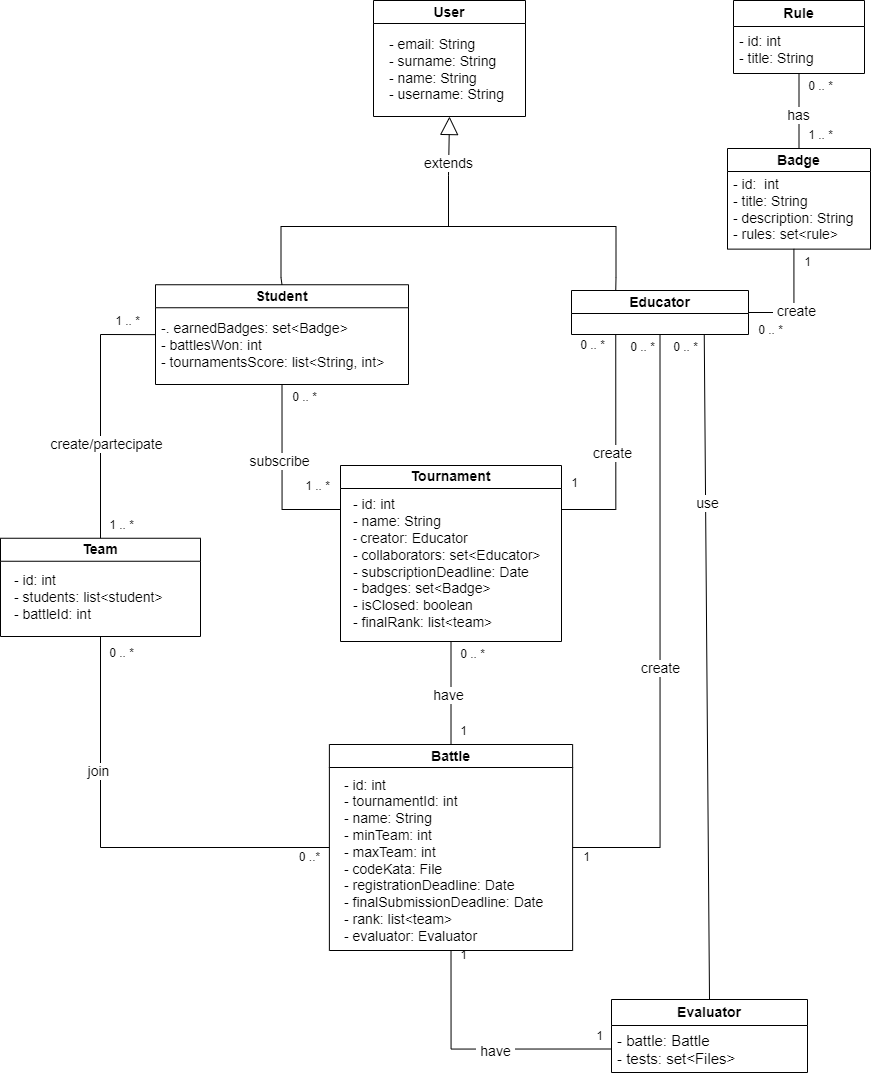
\includegraphics[scale=0.5]{images/class_diagram.png}
    \caption{Domain class diagram}
    \label{fig:class_diagram}
\end{figure}
\clearpage

\subsection{State diagrams}
\clearpage

\subsection{Scenarios}
In this section we will analyze all possible scenarios that can occur in using the CKB platform.

\subsubsection{Scenario 1: Users registration}
Mario is a professor and wants to challenge his students, so he choose the CKB platform. He creates a personal account by inserting some personal information and then get a confirmation e-mail about the creation of a new account. He now can be able to create tournaments and battle. \newline
Peach is a computer science student and wants to improve her software development skills. She learns about the CKB platform from her professor, and decide to create an account to be able to participate to battles. The platform request some personal information and then she get a confirmation e-mail about the creation of his new account. She now have a personal profile where every other user can see her progress, in terms of badges earned, battles won, and tournament rankings. \newline
In both cases the platform request some personal information such as name, surname, username, password, e-mail and the role, that can be student or educator. The account is created after the user clicks on the link sent in the confirmation e-mail. All future notifications will be sent through that e-mail. \newline
Every registered user can log-in with username and password any time, in order to access the personal dashboard and use the CKB platform.

\subsubsection{Scenario 2: Tournament and battle creation}
Mario, that is a registered educator, wants to create a new tournament called "Super Smash". He open the CKB platform, log-in, and from his personal dashboard he select the option "create new tournament". He then follows all the steps that allows him to set a registration deadline and a minimum and maximum number of participants. He can then invite other educators to create battles within his tournament. \newline
Mario invites Luigi to his tournament by adding his username to the list of collaborator. Luigi will be notified by e-mail, and if interested have to join the tournament. \newline
Luigi, that is also a registered educator, wants to create a new battle in Mario's tournament. He open the CKB platform, log-in, and from his personal dashboard he select "Super Smash" from the list of his tournaments.
He then select the option "create new battle" and follows all the steps that allows him to upload the code kata, set a registration deadline, minimum and maximum number of students per group and a final submission deadline.
The tournament "Super Smash" with the first battle are now open, in the list of all ongoing tournaments. \newline
Mario can close the tournament whenever he wants, all ongoing battles will finish within their final submission deadline. Then the CKB platform will publish the final tournament rank when is available and send a notification to all enrolled students.

\subsubsection{Scenario 3: Students team formation}
Peach, that is a registered student, wants to join a tournament. She open the CKB platform, log-in, and from her personal dashboard she is able to see the list of all ongoing tournaments. She selects a tournament and, if the subscription phase is still open, she enrolls.
Daisy enrolls in the same tournament as Peach. \newline
Peach decides to form a team. She can invite students up to the maximum number allowed. She has a limited number of invitations, and if someone does not accept the invitation within a fixed time, she can re-send the invite to someone else.
She sends the invite to Daisy and Toad by adding their username in the team. They will receive a notification by e-mail, and if interested can join the team. Toad decided to join, while Daisy decline the invite. \newline
If the team reach the minimum number of participants for the battle by the registration deadline, they can compete. \newline
\textbf{A team does not reach the minimum number of participants:} Let's say that the minimum number of participant for the  previously mentioned battle is 3, in this case Peach can re-send the invite to another student but she forgot and the registration deadline expires.
Peach's team cannot compete in the battle, therefore their score will be automatically 0.

\subsubsection{Scenario 4: Real-time battle progress}
Peach has formed a valid team for a battle within a tournament. The CKB platform has automatically created a GitHub repository with all the essential elements for the resolution of the battle, and send a link to all enrolled students.
Peach and her team have to fork this repository and set up an automated workflow 
through GitHub Actions. At each pushed commit the platform automatically update the total score of the team. The team is also able to see the current rank evolving during the battle, so they can improve their solution to get a better rank.\newline
\textbf{Students push the solution in a different language:} Every submission that does not use the language specified in the project description will not be evaluated, therefore the team will get a score of 0.  \newline
\textbf{Students push the solution after the deadline:} Every submission after the deadline is ignored, therefore the team will get a score of 0. 

\subsubsection{Scenario 5: Manual evaluation}
After the final submission deadline of a battle expires, a consolidation phase open. During this phase Luigi, that is the creator of the battle, can optionally assign a personal score to each student that will be added to the total score of the entire team.
As soon as Luigi has finished to evaluate all students, he will end the consolidation phase, and when the ranking are available all students will be notified.\newline
\textbf{The score exceed the maximum value:} Luigi can make a mistake and assign a score to a student making the overall team score higher than 100. In this case the score will be automatically cut off to 100.

\subsubsection{Scenario 6: Gamification badges management}
Mario, that is a registered educator, wants to create a new badge that is earned by the student who wrote the most lines of code. From his personal dashboard he select the option "create new badge", then he has to specify the name, a description and one or more rules that regulates if a student is eligible to get that badge. In this case the name will be "Top Writer" and it will be awarded to the student who wrote the most lines of code within a battle. \newline
Peach, that is a student, aspires to earn the "Top Writer" badge, and so she heavily contributed on the last battle. At the end of the battle the CKB platform automatically checks if any student is eligible for a badge, and Peach is assigned the "Top Writer", which will appear on her CKB profile.

\clearpage

\section{Product functions}\label{desc:prodFunc}
In this section are explained the main functions that the CKB should provide to its users.
\subsection{Sign Up and Login}
These function will be available for all user.\newline All users can create a new profile by the sign up function. Each profile is uniquely identified by a username. Each user will be ask to provide an email, a password and role (student or educator). \newline
A login can occur every time by the use of username (or email) and password.

\subsection{Create and manage a tournament}
This function will be available only for educators. \newline
Each educator can create a new tournament and invite other colleagues to create battles within that tournament. At the creation the educator must specify the subscription deadline. 
A tournament can then be closed by its creator, and as soon as the final tournament rank is available the CKB platform notify all students subscribed.

\subsection{Create a battle within a tournament}
This function will be available only for educators. \newline 
An educator can create a new battle in a tournament only if he/she created it or he/she have been invited to collaborate by another colleague.
The system allow the educator to specify: 
\begin{itemize}
    \item code kata, that consist in the description and software project including test cases and build automated scripts.
    \item minimum and maximum number of students per group.
    \item registration deadline.
    \item final submission deadline.
\end{itemize}
The educator has to specify the languages in which the submission can be made.
When the registration deadline expires, the CKB platform creates a GitHub repository that contain the code kata, and sends the link to all the students enrolled in the battle.

\subsection{Subscribe to a tournament}
This function will be available only for students. \newline When a new tournament is created all registered students are notified and can subscribe within a given deadline.

\subsection{Join a battle or a team}
This function will be available only for students. \newline When there is an upcoming battle in a tournament all subscribed students are notified. Each student can join a battle only with a team, even made up of only one student if it is allowed. Teams are formed by invite.

\subsection{Automatic scores updates}
When the students push a new commit into the main branch of the GitHub repository, the CKB platform automatically analyze it and runs the tests to calculate and update the battle score of the team.\newline
The score of each battle is automatically evaluated in the following ways:
\begin{itemize}
        \item functional aspects, measured in terms of number of test cases passed over all test available. The higher the better.
        \item time passed between the registration deadline and the last commit. The lower the better.
        \item quality level of the source, extracted through static analysis tools based on aspects chosen by the educator when creating the battle. 
\end{itemize}

\subsection{Manually scores updates}
When a battle ends, a consolidation stage open. The creator of the battle is able to optionally perform a manual evaluation for each student enrolled.
Once the educator has evaluated all students he can end the consolidation, and when the final battle rank is available all enrolled students will be notified.

\subsection{View all rankings}
Every user can see the list of ongoing tournaments and the corresponding rank (that compares all subscribed students' performance) in the CKB platform.
At the end of each battle the personal tournament score of each student is automatically updated ad the sum of all battle scores received. 

\subsection{View a student profile}
Every user can view a profile of a student by searching for his/her username. In each profile are shown badges earned, battles won, and tournament rankings. 

\subsection{Create and manage gamification badges}
This function will be available only for educators. 
\newline A badge can be created by specifying a title and at least one rule that must be satisfied to achieve it. Each badge is then automatically assigned to one or more students by checking the validity of the rules. Educators can also create new variables that represent relevant information for scoring. A variable is identified by a unique name and a measurement unit, that can be selected by a list of predefined (e.g. integer, float, date, ..).

\section{User characteristics}
Each user must have a profile to be able to use the CKB platform.
There are two different type of users:
\begin{itemize}
	\item \textbf{Students}:
	    The students are the primary users of the CKB platform. They range from beginners to advanced learners. Each student has a personal profile that display their badges earned, battles won, and tournament rankings. 
	\item \textbf{Educators}: 
		The educators can creates and manages tournaments and/or battles. They challenge the students and then evaluate and grade them based on their submissions. An educator must be officially recognized as he/she should have the adequate knowledge.
\end{itemize}

\section{Assumptions, dependencies and constraints}
In this section are listed all assumption made for the domain in which the system operates. These are conditions that the system take for granted because they are external to it but influence its behaviour.

\subsection{Domain assumptions}
\begin{enumerate}[label=\textbf{DA.\arabic*}]
        \item \lbl{da: internet} {Users must have internet connection to interacts with the CKB platform.}
        \item \lbl{da: GitHubAccount} {Students must have a GitHub account to be able to deliver a solution.}
        \item \lbl{da: GitHubFork} {Students must fork the GitHub repository created by the CKB platform and set up an automated workflow through GitHub Actions.}
        \item \lbl{da: autWorkFlow} {The automatic workflow correctly trigger the CKB platform in order to evaluate the new commit.}
        \item \lbl{da: devEnv} {Students must have a development environment with the necessary software tools and libraries to complete code kata battles.}
        \item \lbl{da: eduQual} {Educators must be qualified and experienced in software development and related fields.}
        \item \lbl{da: correctCode} {The uploaded "code kata" by the educators must be correct and complete.}
\end{enumerate}

\subsection{Constraints}
In this section are presented general considerations about limitations on the systems.

\subsubsection{Regulatory policies}
All users information will be processed in according with the GDPR, and e-mail addresses won't be used for commercial purposes.

\subsubsection{Interfaces to other applications}
The CKB platform uses the GitHub API [... to be defined]

	\chapter{Specific Requirements}

\section{External interface Requirements}
\subsection{User Interfaces}
The images below will present an idea of the user interfaces of the major function of the system. Since educators and students uses the platform differently, they will have access to two different personalized dashboard. 
\begin{figure}[H]
        \centering
        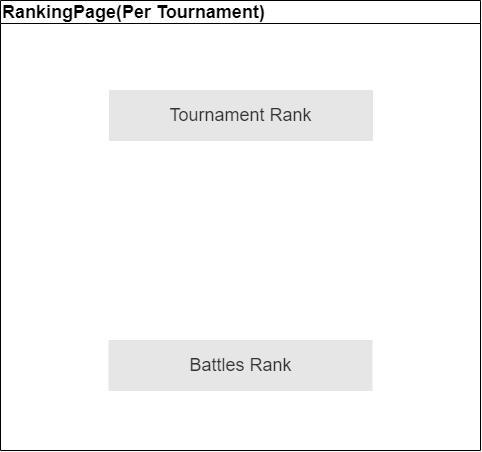
\includegraphics[scale=0.50]{images/interfaces_3.png}
        \caption{Ranking Page}
        \label{fig:rank}
    \end{figure}
    \clearpage
        \begin{figure}[H]
        \centering
        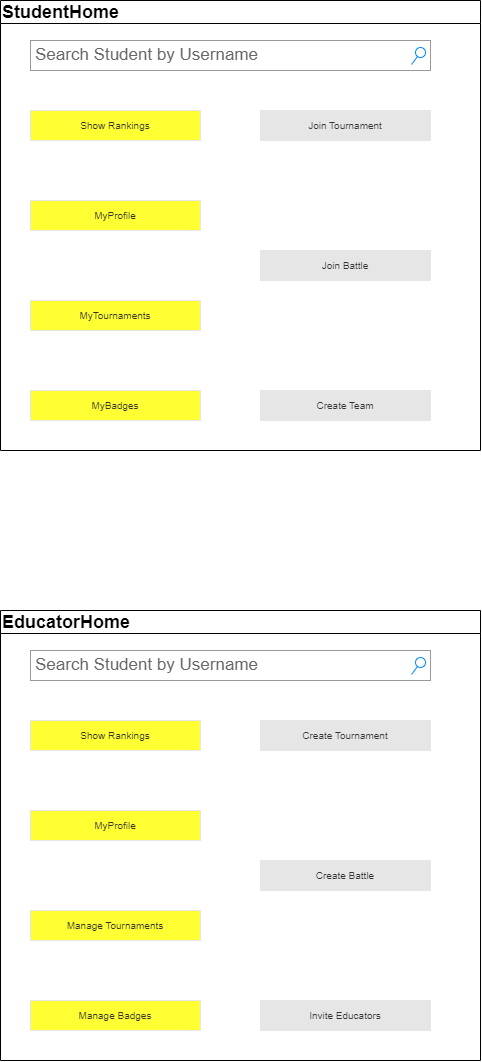
\includegraphics[scale=0.55]{images/interfaces_2.png}
        \caption{Student and Educator Homepage}
        \label{fig:home_pages}
    \end{figure}
    \clearpage

        \begin{figure}[H]
        \centering
        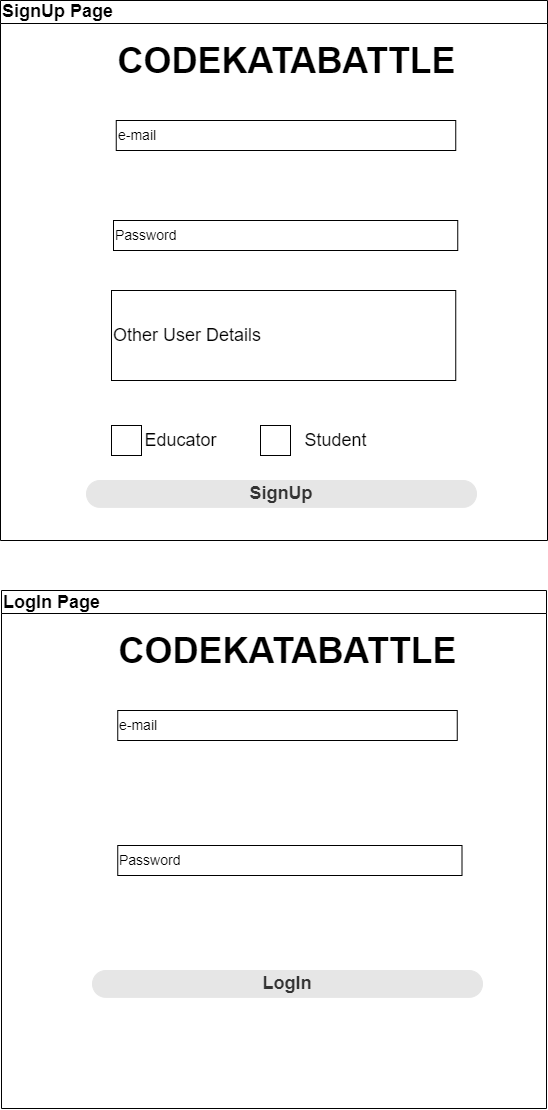
\includegraphics[scale=0.55]{images/interfaces_1 (1).png}
        \caption{Sign Up and Log In Page}
        \label{fig:interfaces_1}
    \end{figure}
    \clearpage
The main differences are in the homepages.(Figure \ref{fig:home_pages})
The grey buttons represent the main operations that the user can do ("Join Tournament, "Create Battle",...), the yellow buttons represent the actions that will be implemented as icons in the homepage.
\subsubsection{Used by the students.}
\subsubsection{Used by the educators.}
\subsection{Hardware Interfaces}
The only hardware interface required is the personal device of the user (computer, tablet or smartphone) that will access the CKB platform through the web browser.
\subsection{Software Interfaces}
The CKB systems uses the GitHub API in order to automatically detects a new commit to the main branch of each forked repository. This will trigger the automated workflow that will evaluate the current submission.
\subsection{Communication Interfaces}
The only communication interface used is internet, via HTTP.
\clearpage

\section{Functional Requirements}
In this section, it is given a complete description of the functional requirements of the system.

    \subsection{Requirements}
        \begin{enumerate}[label=\textbf{R.\arabic*}]
            \subsubsection*{Users}
            \item \lbl{req: reg} {The system shall allow users to register on the platform with their personal information.}
            \item \lbl{req: login} {The system shall allow registered users to log in the platform with valid credentials.}
            \item \lbl{req: listT} {The system shall allow all users to see the list of ongoing tournaments.}
            \item \lbl{req: evalA} {The system shall automatically evaluate submissions.}
            \item \lbl{req: ranks} {The system shall allow users to be able to monitor ranking in real-time during battles and tournaments.}
            \item \lbl{req: profile} {The system shall allow users to see other students' profile.}
            
            \subsubsection*{Educators}
            \item \lbl{req: createT} {The system shall allow the educators to create tournaments.}
            \item \lbl{req: manageT} {The system shall allow the educators to manage their tournaments, in particular invites other collaborators and ends the tournament.}
            \item \lbl{req: createB} {The system shall allow the educators to create code kata battles within a tournament.}
             \item \lbl{req: evalM} {The system shall allow educators to manually evaluate students (if needed) right after a battle closes, during the consolidation stage.}
            \item \lbl{req: createBad} {The system shall allow educators to create badges.}
            \item \lbl{req: defineRV} {The system shall allow educators to define rules and variables.}

            \subsubsection*{Students}
            \item \lbl{req: enrollT} {The system shall allow students to subscribe in tournaments.}
            \item \lbl{req: enrollB} {The system shall allow students to enroll in a battle within a tournament.}
            \item \lbl{req: formTeam} {The system shall allow students to form team for battles, by inviting other students.}        
            \item \lbl{req: notifT} {The system shall notify the students about new tournaments within 10 seconds.}
            \item \lbl{req: notifB} {The system shall notify the students about upcoming battles in tournaments in which they are subscribed within 10 seconds.}
             \item \lbl{req: notifInvite} {The system shall notify the students when they receive an invite to participate in a team within 10 seconds.}
             \item \lbl{req: notifGitHub} {The system shall notify the students when the GitHub repository of a battle is available.}
             \item \lbl{req: notifRankB} {The system shall notify the students when the final battle rank became available within 10 seconds.}
             \item \lbl{req: notifRankT} {The system shall notify the students when the final tournament rank became available within 10 seconds.}
        \end{enumerate}

    \subsection{Goal mapping on requirements and domain assumption}      
        \begin{center}
            \begin{tabular}{ |m{13.5cm}| }
                \hline \\
                \textbf{\print{goal: manageT}} \\
                \hline \\
                \print{req: reg}
                \print{req: login}
                \print{req: createT} 
                \print{req: manageT}
                \print{req: notifT} \\ 
                \hline \\
                \print{da: internet} 
                \print{da: eduQual} \\
                \hline
            \end{tabular} 
        \end{center}
        \begin{center}   
             \begin{tabular}{|m{13.5cm}|}
                \hline \\
                \textbf{\print{goal: createB}} \\
                \hline \\
                \print{req: reg}
                \print{req: login}
                \print{req: createB} 
                \print{req: notifB}\\
                \hline \\
                \print{da: internet} 
                \print{da: correctCode} 
                \print{da: eduQual} \\
                \hline
            \end{tabular} 
        \end{center} 
        \begin{center}
            \begin{tabular}{|m{13.5cm}|}
                \hline \\
                \textbf{\print{goal: enrollT}} \\
                \hline \\
                \print{req: reg}
                \print{req: login}
                \print{req: listT}
                \print{req: enrollT} 
                \print{req: notifT} \\
                \hline \\
                \print{da: internet}\\
                \hline
            \end{tabular} 
        \end{center}
        \begin{center}
            \begin{tabular}{|m{13.5cm}|}
                \hline \\
                \textbf{\print{goal: enrollB}} \\
                \hline \\
                \print{req: reg}
                \print{req: login}
                \print{req: enrollB} 
                \print{req: notifB} 
                \print{req: notifGitHub} \\
                \hline \\
                \print{da: internet} 
                \print{da: GitHubAccount}
                \print{da: devEnv}\\
                \hline
            \end{tabular} 
        \end{center}
        \begin{center}
            \begin{tabular}{|m{13.5cm}|}
                \hline \\
                \textbf{\print{goal: formTeam}} \\
                \hline \\
                \print{req: reg}
                \print{req: login}
                \print{req: formTeam} 
                \print{req: notifInvite} \\
                \hline \\
                \print{da: GitHubAccount}
                \print{da: devEnv}
                \print{da: GitHubFork}
                \print{da: internet} \\
                \hline
            \end{tabular} 
        \end{center}
        \begin{center}
            \begin{tabular}{|m{13.5cm}|}
                \hline \\
                \textbf{\print{goal: scoreB}} \\
                \hline \\
                \print{req: reg}
                \print{req: login}
                \print{req: evalA} 
                \print{req: evalM} 
                \print{req: ranks} 
                \print{req: notifRankB} \\
                \hline \\
                \print{da: internet} 
                \print{da: autWorkFlow}\\
                \hline
            \end{tabular} 
        \end{center}
        \begin{center}
            \begin{tabular}{|m{13.5cm}|}
                \hline \\
                \textbf{\print{goal: listT}} \\
                \hline \\
                \print{req: reg}
                \print{req: login}
                \print{req: listT} 
                \print{req: notifT}\\
                \hline \\
                \print{da: internet} \\
                \hline
            \end{tabular} 
        \end{center}
        \begin{center}
            \begin{tabular}{|m{13.5cm}|}
                \hline \\
                \textbf{\print{goal: rankT}} \\
                \hline \\
                \print{req: reg}
                \print{req: login}
                \print{req: ranks} 
                \print{req: notifRankT} \\
                \hline \\
                \print{da: internet} \\
                \hline
            \end{tabular} 
        \end{center}
        \begin{center}
            \begin{tabular}{|m{13.5cm}|}
                \hline \\
                \textbf{\print{goal: createBad}} \\
                \hline \\
                \print{req: reg}
                \print{req: login}
                \print{req: createBad}
                \print{req: defineRV}\\
                \hline \\
                \print{da: internet} 
                \print{da: eduQual}\\
                \hline
            \end{tabular} 
        \end{center}
        \begin{center}
            \begin{tabular}{|m{13.5cm}|}
                \hline \\
                \textbf{\print{goal: profile}} \\
                \hline \\
                \print{req: reg}
                \print{req: login}
                \print{req: profile} \\
                \hline \\
                \print{da: internet} \\
                \hline
            \end{tabular} 
        \end{center}
    \clearpage
    
    \subsection{Use cases}
    In figure \ref{fig:use_cases_diagram} is represented a general overview of all use cases deduced from the scenarios in section \ref{desc:scenarios}. All cases include "User login" because all function provided by the platform are accessible to registered users. (except for use registration)
    \begin{figure}[H]
        \centering
        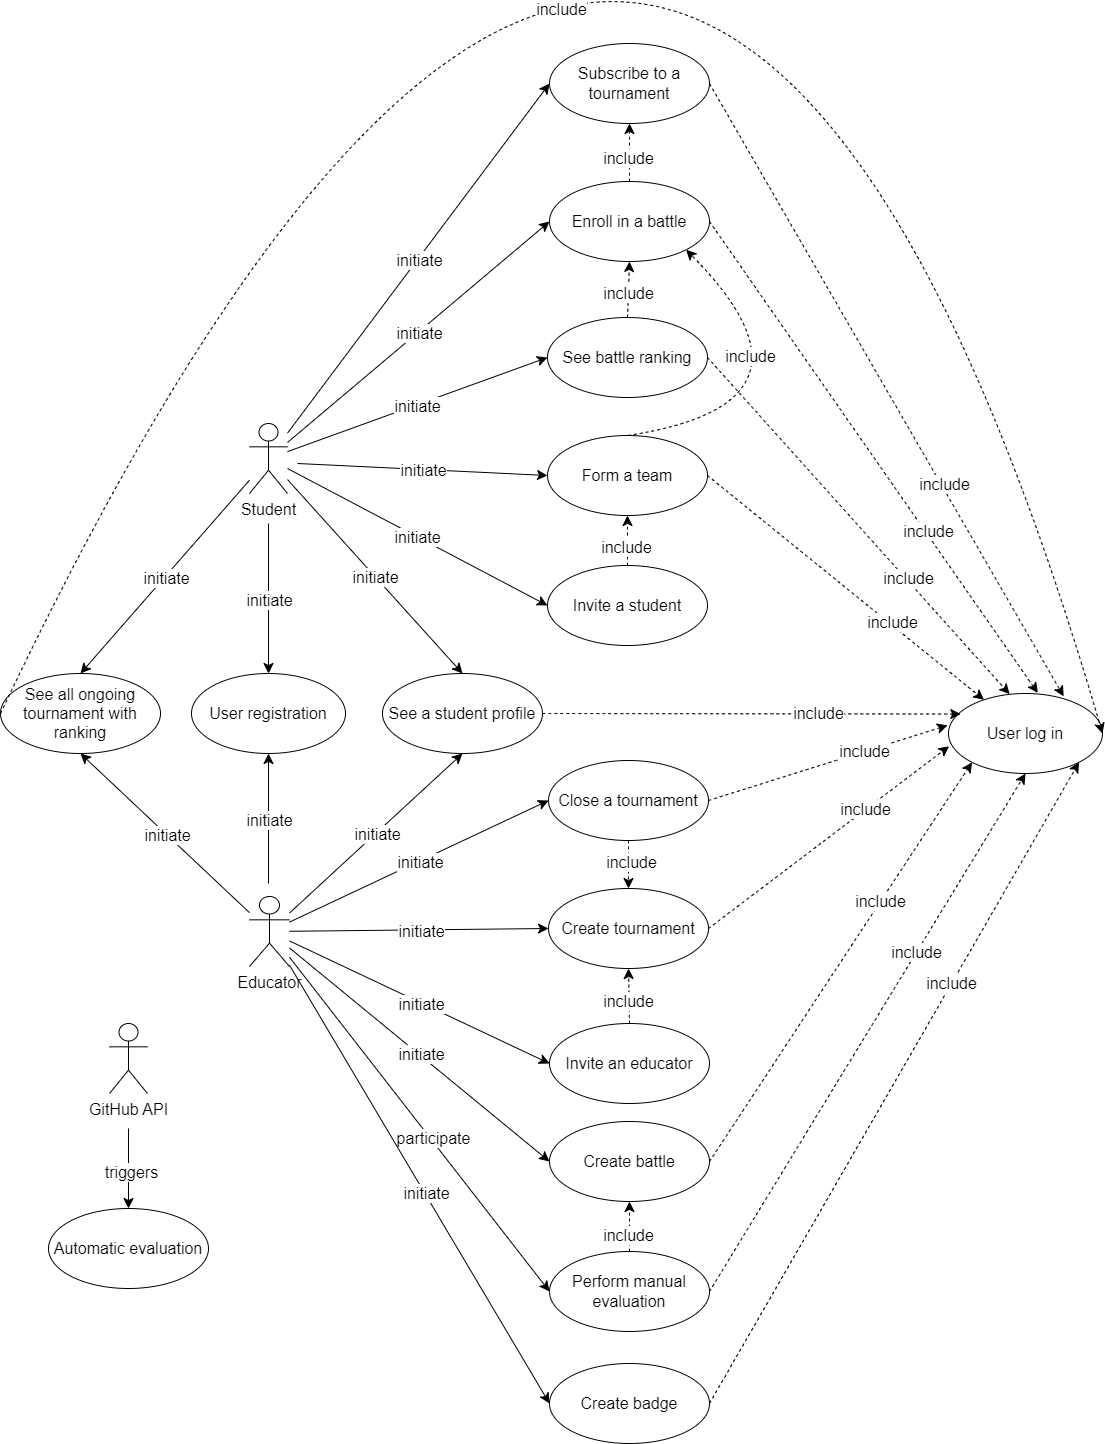
\includegraphics[scale=0.35]{images/use_cases_diagram.png}
        \caption{Use cases diagram}
        \label{fig:use_cases_diagram}
    \end{figure}
    \clearpage
    
    \begin{enumerate}[label=\textbf{UC.\arabic*}]
        \item \lbl{uc: reg} \textbf{User registration}
        \begin{table}[H]
    	    \centering
                \renewcommand{\arraystretch}{1.5}
                \begin{tabular}{|m{3.2cm}|m{9.8cm}|}
                    \hline
                    \textbf{Name} & User registration. \\
                    \hline
                    \textbf{Actors} & Educators, Students. \\
                    \hline
                    \textbf{Entry conditions}  & An user enters the CKB platform for the first time. \\
                    \hline
                    \textbf{Event flow}  & 
                    \begin{enumerate}[label=\arabic*.]
                        \item The user visualize the register page.
                        \item The user inserts the requested personal information.
                        \item The user clicks on the "sign up" button.
                        \item The system checks if the username is available.
                        \item The system sends a confirmation e-mail to the user.
                        \item The user clicks on the link on the confirmation e-mail received.
                        \item The system creates the personal profile of the user.
                    \end{enumerate}\\
                    \hline
                    \textbf{Exit conditions}  & The user is registered in the system. \\
                    \hline
                    \textbf{Exceptions}  & 
                    \begin{itemize}
                        \item If the chosen username is not available the system will throw an error message and the user will be requested to choose another one.
                    \end{itemize} \\
                    \hline 
                \end{tabular}
        \end{table}
        \item \lbl{uc: login} \textbf{User login}
        \begin{table}[H]
    	    \centering
                \renewcommand{\arraystretch}{1.5}
                \begin{tabular}{|m{3.2cm}|m{9.8cm}|}
                    \hline
                    \textbf{Name} & User login.\\
                    \hline
                    \textbf{Actors} &  Educators, students. \\
                    \hline
                    \textbf{Entry conditions}  & The user opens the CKB platform and clicks on "log in" button. \\
                    \hline
                    \textbf{Event flow}  & 
                    \begin{enumerate}[label=\arabic*.]
                        \item The user visualize the log in page.
                        \item The user inserts username and password in the form.
                        \item The user clicks on "log in" button.
                        \item The system checks the credentials.
                        \item The system show the personal dashboard.
                    \end{enumerate}\\
                    \hline
                    \textbf{Exit conditions}  & The user has entered the CKB platform successfully. \\
                    \hline
                    \textbf{Exceptions}  & If username and/or password are not correct the system will throw an error message and return to the entry condition. \\
                    \hline 
                \end{tabular}
        \end{table}
        \item \lbl{uc: createT} \textbf{Create a tournament}
        \begin{table}[H]
    	    \centering
                \renewcommand{\arraystretch}{1.5}
                \begin{tabular}{|m{3.2cm}|m{9.8cm}|}
                    \hline
                    \textbf{Name} & Create a tournament. \\
                    \hline
                    \textbf{Actors} & Educators. \\
                    \hline
                    \textbf{Entry conditions}  & An educator, who is logged in the platform, clicks on the button "create tournament". \\
                    \hline
                    \textbf{Event flow}  &  
                    \begin{enumerate}[label=\arabic*.]
                        \item The educator inserts all needed information in the form.
                        \item The system checks that the correctness of all information.
                    \end{enumerate}\\
                    \hline
                    \textbf{Exit conditions}  & The tournament has been successfully created and can be visualize in the list of all ongoing tournaments. All registered students will receive a notification that a new tournament is available.\\
                    \hline
                    \textbf{Exceptions}  & 
                    If there are some incorrect information, the system will throw an error message and the educator will be requested to modify it. The system return to the entry condition. \\
                    \hline 
                \end{tabular}
        \end{table}
        \item \lbl{uc: createB} \textbf{Create battle}
        \begin{table}[H]
    	    \centering
                \renewcommand{\arraystretch}{1.5}
                \begin{tabular}{|m{3.2cm}|m{9.8cm}|}
                    \hline
                    \textbf{Name} & Create a battle. \\
                    \hline
                    \textbf{Actors} & Educators. \\
                    \hline
                    \textbf{Entry conditions}  &  An educator, who is logged in the platform, wants to create a battle.\\
                    \hline
                    \textbf{Event flow}  & 
                    \begin{enumerate}[label=\arabic*.]
                        \item The educator clicks on the button "my tournaments".
                        \item The educator visualize a list of tournaments to which he/she has access.
                        \item The educator select a tournament from the list.
                        \item The educator clicks on the button "create battle".
                        \item The educator inserts all needed information in the form.
                        \item The system checks that the correctness of all information.
                    \end{enumerate}\\
                    \hline
                    \textbf{Exit conditions}  & The battle has been successfully created and all students subscribed to the tournament in which it belongs have received a notification.  \\
                    \hline
                    \textbf{Exceptions}  &  If there are some incorrect information, the system will throw an error message and the educator will be requested to modify it.  The system return to the entry condition. \\
                    \hline 
                \end{tabular}
        \end{table}
        \item \lbl{uc: inviteE} \textbf{Invite an educator}
        \begin{table}[H]
    	    \centering
                \renewcommand{\arraystretch}{1.5}
                \begin{tabular}{|m{3.2cm}|m{9.8cm}|}
                    \hline
                    \textbf{Name} & Invite an educator. \\
                    \hline
                    \textbf{Actors} & Educators. \\
                    \hline
                    \textbf{Entry conditions}  & An educator, who created a tournament, wants to invite some colleagues to participate. \\
                    \hline
                    \textbf{Event flow}  & 
                    \begin{enumerate}[label=\arabic*.]
                        \item The educator clicks on the button "my tournaments".
                        \item The educator visualize a list of tournaments to which he/she has access.
                        \item The educator select a tournament from the list.
                        \item The educator clicks on the button "invite educator"
                        \item The educator insert the username of the colleague he/she wants to invite.
                        \item The system sends an e-mail to the selected colleague.
                    \end{enumerate}\\
                    \hline
                    \textbf{Exit conditions}  & The invite has been successfully sent. \\
                    \hline
                    \textbf{Exceptions} & If the selected username does not exist or belongs to a student the system will throw an error message. The system will return to the entry conditions.
                \end{tabular}
        \end{table}
        \item \lbl{uc: closeT} \textbf{Close a tournament}
        \begin{table}[H]
    	    \centering
                \renewcommand{\arraystretch}{1.5}
                \begin{tabular}{|m{3.2cm}|m{9.8cm}|}
                    \hline
                    \textbf{Name} & Close a tournament. \\
                    \hline
                    \textbf{Actors} & Educators. \\
                    \hline
                    \textbf{Entry conditions}  &  An educator, who created a tournament, wants close it. \\
                    \hline
                    \textbf{Event flow}  & 
                    \begin{enumerate}[label=\arabic*.]
                        \item The educator clicks on the button "my tournaments"
                        \item The educator visualize a list of tournaments to which he/she has access.
                        \item The educator select a tournament from the list.
                        \item The educator clicks on the button "close tournament".
                        \item The system checks whether all battles in that tournament are finished.
                    \end{enumerate}\\
                    \hline
                    \textbf{Exit conditions}  & The tournament has been successfully closed. \\
                    \hline
                    \textbf{Exceptions}  & If not all battles of the tournament are over, the system will throw an error message and the educator will not be able to close the tournament. The system returns to the entry condition.\\
                    \hline 
                \end{tabular}
        \end{table}
        \item \lbl{uc: rankT} \textbf{Visualize all ongoing tournament with ranking}
        \begin{table}[H]
    	    \centering
                \renewcommand{\arraystretch}{1.5}
                \begin{tabular}{|m{3.2cm}|m{9.8cm}|}
                    \hline
                    \textbf{Name} & Visualize all ongoing tournament with ranking.  \\
                    \hline
                    \textbf{Actors} & Educators and students. \\
                    \hline
                    \textbf{Entry conditions}  & A user wants to see the list of all tournaments and/or their rankings. \\
                    \hline
                    \textbf{Event flow}  & 
                    \begin{enumerate}[label=\arabic*.]
                        \item The user clicks on the button "see all tournaments"
                        \item The user visualize a list of tournaments.
                        \item The user clicks on a tournament to visualize its ranking.
                    \end{enumerate}\\
                    \hline
                    \textbf{Exit conditions}  & The user visualize a list of tournaments and/or a specific ranking. \\
                    \hline
                \end{tabular}
        \end{table}
        \item \lbl{uc: enrollT} \textbf{Subscribe to a tournament}
        \begin{table}[H]
    	    \centering
                \renewcommand{\arraystretch}{1.5}
                \begin{tabular}{|m{3.2cm}|m{9.8cm}|}
                    \hline
                    \textbf{Name} & Subscribe to a tournament.\\
                    \hline
                    \textbf{Actors} & Students. \\
                    \hline
                    \textbf{Entry conditions}  & A student, who is registered to the platform, receive a notification that a new tournament is available and wants to subscribe.\\
                    \hline
                    \textbf{Event flow}  & 
                    \begin{enumerate}[label=\arabic*.]
                        \item The user clicks on the link received via e-mail.
                        \item The system check if the subscription deadline is not expired.
                    \end{enumerate}\\ 
                    \hline
                    \textbf{Exit conditions}  & The student is successfully subscribed to the tournament. The system will send the student further notification about the upcoming battles. \\
                    \hline
                    \textbf{Exceptions}  & If the subscription deadline is expired, the system will throw an error message and the student will not be able to subscribe to the tournament. The system will return to the entry condition. \\
                    \hline 
                \end{tabular}
        \end{table}
        \item \lbl{uc: enrollB} \textbf{Enroll in a battle}
        \begin{table}[H]
    	    \centering
                \renewcommand{\arraystretch}{1.5}
                \begin{tabular}{|m{3.2cm}|m{9.8cm}|}
                    \hline
                    \textbf{Name} & Enroll in a battle. \\
                    \hline
                    \textbf{Actors} & Students. \\
                    \hline
                    \textbf{Entry conditions}  & A student, who is subscribed to a tournament, receive a notification that a new battle is available and wants to enroll.\\
                    \hline
                    \textbf{Event flow}  & 
                    \begin{enumerate}[label=\arabic*.]
                        \item The student clicks on the link received by e-mail.
                        \item The system checks if the registration deadline is not expired.
                    \end{enumerate}\\ 
                    \hline
                    \textbf{Exit conditions}  & The student is successfully enrolled to the battle. \\
                    \hline
                    \textbf{Exceptions}  & If the registration deadline is expired, the system will throw an error message and the student will not be able to subscribe to the battle. The system will return to the list of battles.  \\
                    \hline 
                \end{tabular}
        \end{table}
        \item \lbl{uc: inviteS} \textbf{Invite a student}
        \begin{table}[H]
    	    \centering
                \renewcommand{\arraystretch}{1.5}
                \begin{tabular}{|m{3.2cm}|m{9.8cm}|}
                    \hline
                    \textbf{Name} & Invite a student. \\
                    \hline
                    \textbf{Actors} & Students. \\
                    \hline
                    \textbf{Entry conditions}  & A student, who is enrolled in a battle, wants to create a team. \\
                    \hline
                    \textbf{Event flow}  &  
                    \begin{enumerate}[label=\arabic*.]
                        \item The student clicks on the button "my battles".
                        \item The student visualizes the list of battles he/she is registered to.
                        \item The student selects a battle.
                        \item The student visualizes his/hers current team.
                        \item The student clicks on the button "invite a student".
                        \item The system checks if the registration deadline is not expired.
                        \item The student inserts the username of the student who he/she wants to invite.
                        \item The system checks if the username inserted is enrolled in the battle.
                    \end{enumerate}\\ 
                    \hline
                    \textbf{Exit conditions}  & The invited student has received an e-mail. \\
                    \hline
                    \textbf{Exceptions}  &
                    \begin{itemize}
                        \item If the registration deadline for the battle is expired, the invite will not be sent.
                        \item If the invited student is not enrolled in the invite will not be sent.
                    \end{itemize} 
                     In both cases the system will throw an error message and return to the entry condition.\\
                    \hline 
                \end{tabular}
        \end{table}
        \item \lbl{uc: leaveT} \textbf{Leave a team}
        \begin{table}[H]
    	    \centering
                \renewcommand{\arraystretch}{1.5}
                \begin{tabular}{|m{3.2cm}|m{9.8cm}|}
                    \hline
                    \textbf{Name} & Leave a team. \\
                    \hline
                    \textbf{Actors} & Students. \\
                    \hline
                    \textbf{Entry conditions}  & A student wants to leave his/hers current team. \\
                    \hline
                    \textbf{Event flow}  & 
                    \begin{enumerate}[label=\arabic*.]
                        \item The student clicks on the button "my battles".
                        \item The student visualizes the list of battles he/she is registered to.
                        \item The student selects a battle.
                        \item The student visualizes his/hers current team.
                         \item The student clicks on the button "leave team".
                        \item The system check if the registration deadline is not expired.
                    \end{enumerate}\\ 
                    \hline
                    \textbf{Exit conditions}  & The student has successfully left his/her team. \\
                    \hline
                    \textbf{Exceptions}  & If the registration deadline is already expired the system will throw an error message and the student will not be able to leave the team. The system will return to the entry condition. \\
                    \hline 
                \end{tabular}
        \end{table}
        \item \lbl{uc: rankB} \textbf{View battle ranking}
        \begin{table}[H]
    	    \centering
                \renewcommand{\arraystretch}{1.5}
                \begin{tabular}{|m{3.2cm}|m{9.8cm}|}
                    \hline
                    \textbf{Name} & View battle ranking. \\
                    \hline
                    \textbf{Actors} & Educators and students. \\
                    \hline
                    \textbf{Entry conditions}  & An user wants to see the real-time ranking of a battle. \\
                    \hline
                    \textbf{Event flow}  & 
                    \begin{enumerate}[label=\arabic*.]
                        \item The user clicks on the button "my battles".
                        \item The user visualizes the list of battles that are correlated to him/her.
                        \item The user selects a battle.
                        \item The system show the real-time raking of the selected battle.
                    \end{enumerate}\\ 
                    \hline
                    \textbf{Exit conditions}  & The user visualize the real-time ranking of a battle. \\
                    \hline
                \end{tabular}
        \end{table}
        \item \lbl{uc: evalM} \textbf{Perform manual evaluation}
        \begin{table}[H]
    	    \centering
                \renewcommand{\arraystretch}{1.5}
                \begin{tabular}{|m{3.2cm}|m{9.8cm}|}
                    \hline
                    \textbf{Name} & Perform manual evaluation. \\
                    \hline
                    \textbf{Actors} & Educators. \\
                    \hline
                    \textbf{Entry conditions}  & An educator wants to manually evaluate some students. \\
                    \hline
                    \textbf{Event flow}  & 
                    \begin{enumerate}[label=\arabic*.]
                        \item The educator clicks on the button "my battles".
                        \item The educator visualize the list of battles that are correlated to him/her.
                        \item The educator select the battle he/she wants to evaluate.
                        \item The educator clicks on the button "perform manual evaluation".
                        \item The educator assigns a personal score to each participant in the battle.
                        \item The educator clicks on the button "end consolidation stage".
                    \end{enumerate}\\ 
                    \hline
                    \textbf{Exit conditions}  &  The educator end the consolidation stage. \\
                    \hline
                \end{tabular}
        \end{table}
        \item \lbl{uc: evalA} \textbf{Perform automatic evaluation}
        \begin{table}[H]
    	    \centering
                \renewcommand{\arraystretch}{1.5}
                \begin{tabular}{|m{3.2cm}|m{9.8cm}|}
                    \hline
                    \textbf{Name} & Perform automatic evaluation. \\
                    \hline
                    \textbf{Actors} & GitHub API. \\
                    \hline
                    \textbf{Entry conditions}  & A team push a new solution on the GitHub repository. \\
                    \hline
                    \textbf{Event flow}  & 
                    \begin{enumerate}[label=\arabic*.]
                        \item The GitHub API triggers the CKB platform.
                        \item The system perform the automatic evaluation.
                        \item The system update the score of each team and the real-time rank.
                    \end{enumerate}\\ 
                    \hline
                    \textbf{Exit conditions}  &  The real-time rank is updated. \\
                    \hline
                \end{tabular}
        \end{table}
        \item \lbl{uc: createBadge} \textbf{Create a badge}
        \begin{table}[H]
    	    \centering
                \renewcommand{\arraystretch}{1.5}
                \begin{tabular}{|m{3.2cm}|m{9.8cm}|}
                    \hline
                    \textbf{Name} & Create a badge. \\
                    \hline
                    \textbf{Actors} & Educators. \\
                    \hline
                    \textbf{Entry conditions}  & An educator wants to create a new badge. \\
                    \hline
                    \textbf{Event flow}  & 
                    \begin{enumerate}[label=\arabic*.]
                        \item The user clicks on the button "create badge".
                        \item The user inserts all information requested.
                        \item The system check the inserted information.
                    \end{enumerate}\\ 
                    \hline
                    \textbf{Exit conditions}  & The badge has been successfully created. \\
                    \hline
                \end{tabular}
        \end{table}
        \item \lbl{uc: profile} \textbf{See student profile}
        \begin{table}[H]
    	    \centering
                \renewcommand{\arraystretch}{1.5}
                \begin{tabular}{|m{3.2cm}|m{9.8cm}|}
                    \hline
                    \textbf{Name} & See student profile. \\
                    \hline
                    \textbf{Actors} & Educators and students. \\
                    \hline
                    \textbf{Entry conditions}  & An user wants to see a personal profile of a student. \\
                    \hline
                    \textbf{Event flow}  & 
                    \begin{enumerate}[label=\arabic*.]
                        \item The user clicks on the button "see student profile".
                        \item The user inserts the username of the student he/she wants to see.
                        \item The system check the inserted information.
                        \item The system show the personal profile requested if present.
                    \end{enumerate}\\ 
                    \hline
                    \textbf{Exit conditions}  & The user see the personal profile of a student. \\
                    \hline
                    \textbf{Exceptions} & If the selected username does not exist the system will throw an error message. The system will return to the entry conditions \\
                    \hline
                \end{tabular}
        \end{table}
    \end{enumerate}
    

    \subsection{Traceability matrix}
    \begin{table}[h]
	    \centering
            \renewcommand{\arraystretch}{1.5}
            \begin{tabular}{|m{3cm}|m{3cm}|m{3cm}|m{3cm}|}
                \hline
                \textbf{Use Case ID} & \textbf{Goal ID} & \textbf{Req ID} & \textbf{Scenarios} \\
                \hline
                \ref{uc: reg} & ALL & \ref{req: reg} & sce1  \\
                \hline
                \ref{uc: login} & ALL & \ref{req: login} & sce1  \\
                \hline
                \ref{uc: createT} & \ref{goal: manageT} & \ref{req: createT} & sce2  \\
                \null & \null  & \ref{req: manageT}&\null \\
                \null & \null  & \ref{req: notifT}&\null \\
                \hline
                \ref{uc: createB} & \ref{goal: createB} & \ref{req: createB} & sce2  \\
                \null & \null  & \ref{req: notifB}&\null \\
                \hline
                \ref{uc: inviteE} & \ref{goal: createB} & \ref{req: manageT} & sce2  \\
                \hline
                \ref{uc: closeT} & \ref{goal: manageT} & TO DEFINE & sce2  \\
                \hline
                \ref{uc: rankT} & \ref{goal: listT} & \ref{req: listT} & sce4  \\
                \null & \null  & \ref{req: notifT}&\null \\
                \null & \ref{goal: rankT}  & \ref{req: ranks}&\null \\
                \null & \null  & \ref{req: notifRankT}&\null \\
                \hline
                \ref{uc: enrollT} & \ref{goal: enrollT} & \ref{req: listT} & sce2  \\
                \null & \null  & \ref{req: enrollT}&\null \\
                \null & \null  & \ref{req: notifT}&\null \\
                \hline
                \ref{uc: enrollB} & \ref{goal: enrollB} & \ref{req: enrollB} & sce3 \\
                \null & \null  & \ref{req: formTeam}& \null \\ 
                \null & \null  & \ref{req: notifB}&\null \\
                \null & \null  & \ref{req: notifGitHub}&\null \\
                \hline
                \ref{uc: inviteS} & \ref{goal: formTeam} & \ref{req: formTeam} & sce3 \\
                \null & \null  & \ref{req: notifInvite}& \null \\ 
                \hline
                \ref{uc: leaveT} & \ref{goal: formTeam} & \ref{req: formTeam} & sce3 \\
                \null & \null  & \ref{req: notifInvite}& \null \\ 
                \hline
                \ref{uc: rankB} & \ref{goal: scoreB} & \ref{req: evalA} & sce4 \\
                \null & \null  & \ref{req: ranks}& \null \\ 
                \null & \null  & \ref{req: evalM}&\null \\
                \null & \null  & \ref{req: notifRankB}&\null \\
                \hline
                \ref{uc: evalM} & \ref{goal: scoreB} & \ref{req: evalM} & sce5 \\
                \null & \null  & \ref{req: notifRankB}&\null \\
                \hline
                \ref{uc: evalA} & \ref{goal: scoreB} & \ref{req: evalA} & sce4 \\
                \null & \null  & \ref{req: ranks}&\null \\
                \null & \null  & \ref{req: notifRankB}&\null \\
                \hline

            \end{tabular}
    \end{table}

    \clearpage
    \begin{table}[h]
        \centering
        \renewcommand{\arraystretch}{1.5}
        \begin{tabular}{|m{3cm}|m{3cm}|m{3cm}|m{3cm}|}
            \hline
            \textbf{Use Case ID} & \textbf{Goal ID} & \textbf{Req ID} & \textbf{Scenarios} \\
            \hline
            \ref{uc: createBadge} & \ref{goal: createBad} & \ref{req: createBad} & sce6 \\
            \null & \null  & \ref{req: defineRV}&\null \\
            \hline
            \ref{uc: profile} & \ref{goal: profile} & \ref{req: profile} & sce7 \\
            \hline
        \end{tabular}
    \end{table}
    
\clearpage
\section{Performance Requirements}
In this section are listed some performance requirements for the CKB platform that are essential to the efficiency of the entire system.
The CKB platform should be able to guarantee the connection of 100.000 users simultaneously. \newline 
In less than 2 seconds, it should be able to respond to user interactions, such as page loading. \newline
In less than 5 seconds, it should be able to send a response to a query and run its algorithms on the metadata. This is crucial for having real-time evaluation of the students' submissions.

\section{Design Constraints}
\subsection{Standards Compliance}
The code should follow the requirements contained in this document. Furthermore, its comments should
be clear and focused.
The system will store in the database 3 types of data:
\begin{enumerate}
    \item User main information for example email-Password as primary key, name , surname...
    \item The final rankings of a tournament. The system saves in the database the ranking of a tournament once it's finished.
    \item The final ranking of a battle.
\end{enumerate}

CKB system shall use stateless protocols and standard operations to allow components to
be managed and updated without affecting the system as a whole.
It’s crucial to design modules properly so that ease of use, security and performance will
remain the core factors of the system.
\subsection{Hardware Limitations}
To use CKB the user needs to have a device that's at least can connect to internet and can share code on GitHub.
The device might be connected to internet and to the GitHub account that the user put during the registration. 
\subsection{Other Constraints}
CKB system will send emails to the users and automatically pulls the GitHub main branch of the teams so it's important that the user allows the system to send emails and to join the GitHub project.

\section{Software System Attributes}
\subsection{Reliability}
The CKB platform should be highly reliable in order to guarantee the continuity of the service, every user should be able to access the platform anytime. The system should implements robust errors handling and fault tolerance mechanism to prevent error propagation and data loss. \subsection{Availability}
The CKB platform should be available to users 24/7, without frequent interruptions. 
Since the system is not emergency-related, it should be up 99\% of the time.
This means that the average downtime is around at 3.65 days per year. \newline
In order to achieve this level of availability the system should implement a disaster recovery plan, monitoring and alerting tools, and the ability to react fast to resolve any system issues.
\subsection{Security}
As the system store some personal information about the users, security is an important issue. This stored data must be encrypted, and passwords must also be hashed. \newline
Every time a password need to be recovered a new one must be created, by sending a verification e-mail that contain a time-limited that confirm the user identity and gives them access to reset their password.
\subsection{Maintainability}
The CKB system should be divided in different modules implementing the various functionalities. In this way ordinary maintenance and/or future fixes or improvements will be easier to be performed. \newline
Maintenance and updates must be scheduled in advance so that they do not interfere with ongoing battles. 
\subsection{Portability}
The CKB platform should be accessible from any web browser.
\subsection{Usability}
The user interfaces of the platform should be easy to use and intuitive.

\section{Other Requirements}
\subsection{Privacy Requirements}
At the registration every user is asked to fill the following mandatory fields:
name, surname and e-mail. 

	\chapter{Formal Analysis Using Alloy}

\section{Alloy Model}
In this section is presented a formal model of the CKB platform using alloy. The model is a simplification of the entire system and represent only the most significant parts.
\lstinputlisting[language=alloy]{CKBmodel.als}
	\chapter{Effort Spent}

\section{Teamwork}
\begin{center}
    \begin{tabular}{@{}p{0.5\linewidth} p{0.2\linewidth}@{}}
        \hline
        \textbf{Task} & \textbf{Hours} \\ \hline
        Initial briefing & 2 \\ \hline
    \end{tabular}
\end{center}

\section{Eliahu Itamar Cohen}
\begin{center}
    \begin{tabular}{@{}p{0.5\linewidth} p{0.2\linewidth}@{}}
        \hline
        \textbf{Task} & \textbf{Hours} \\ \hline
        Chapter 1: Introduction & 0 \\ \hline
        Chapter 2: Overall description & 1.5 \\ \hline
        Chapter 3: Specific requirements & 1 \\ \hline
        Chapter 4: Alloy & 0 \\ \hline
        Extra Activities & 2 \\ \hline
    \end{tabular}
\end{center}

\section{Marco Gervatini}
\begin{center}
	\begin{tabular}{@{}p{0.5\linewidth} p{0.2\linewidth}@{}}
		\hline
		\textbf{Task} & \textbf{Hours} \\ \hline
            Chapter 1: Introduction & 0 \\ \hline
            Chapter 2: Overall description & 1.5 \\ \hline
            Chapter 3: Specific requirements & 0 \\ \hline
            Chapter 4: Alloy & 0 \\ \hline
            Extra Activities & 2 \\ \hline
	\end{tabular}
\end{center}

\section{Caterina Motti}
\begin{center}
	\begin{tabular}{@{}p{0.5\linewidth} p{0.2\linewidth}@{}}
		\hline
		\textbf{Task} & \textbf{Hours} \\ \hline
            Document setup & 2 \\ \hline
            Chapter 1: Introduction & 3 \\ \hline
            Chapter 2: Overall description & 10.5 \\ \hline
            Chapter 3: Specific requirements & 8 \\ \hline
            Chapter 4: Alloy & 0 \\ \hline
            Extra Activities & 1 \\ \hline
	\end{tabular}
\end{center}

        \chapter{References}
\begin{itemize}
    \item All diagrams have been made with \url{https://www.draw.io}
    \item Alloy code development has been supported by VS code (Extensions used: Alloy, Alloy VSCode) and Alloy Analyzer
\end{itemize}

\end{document}